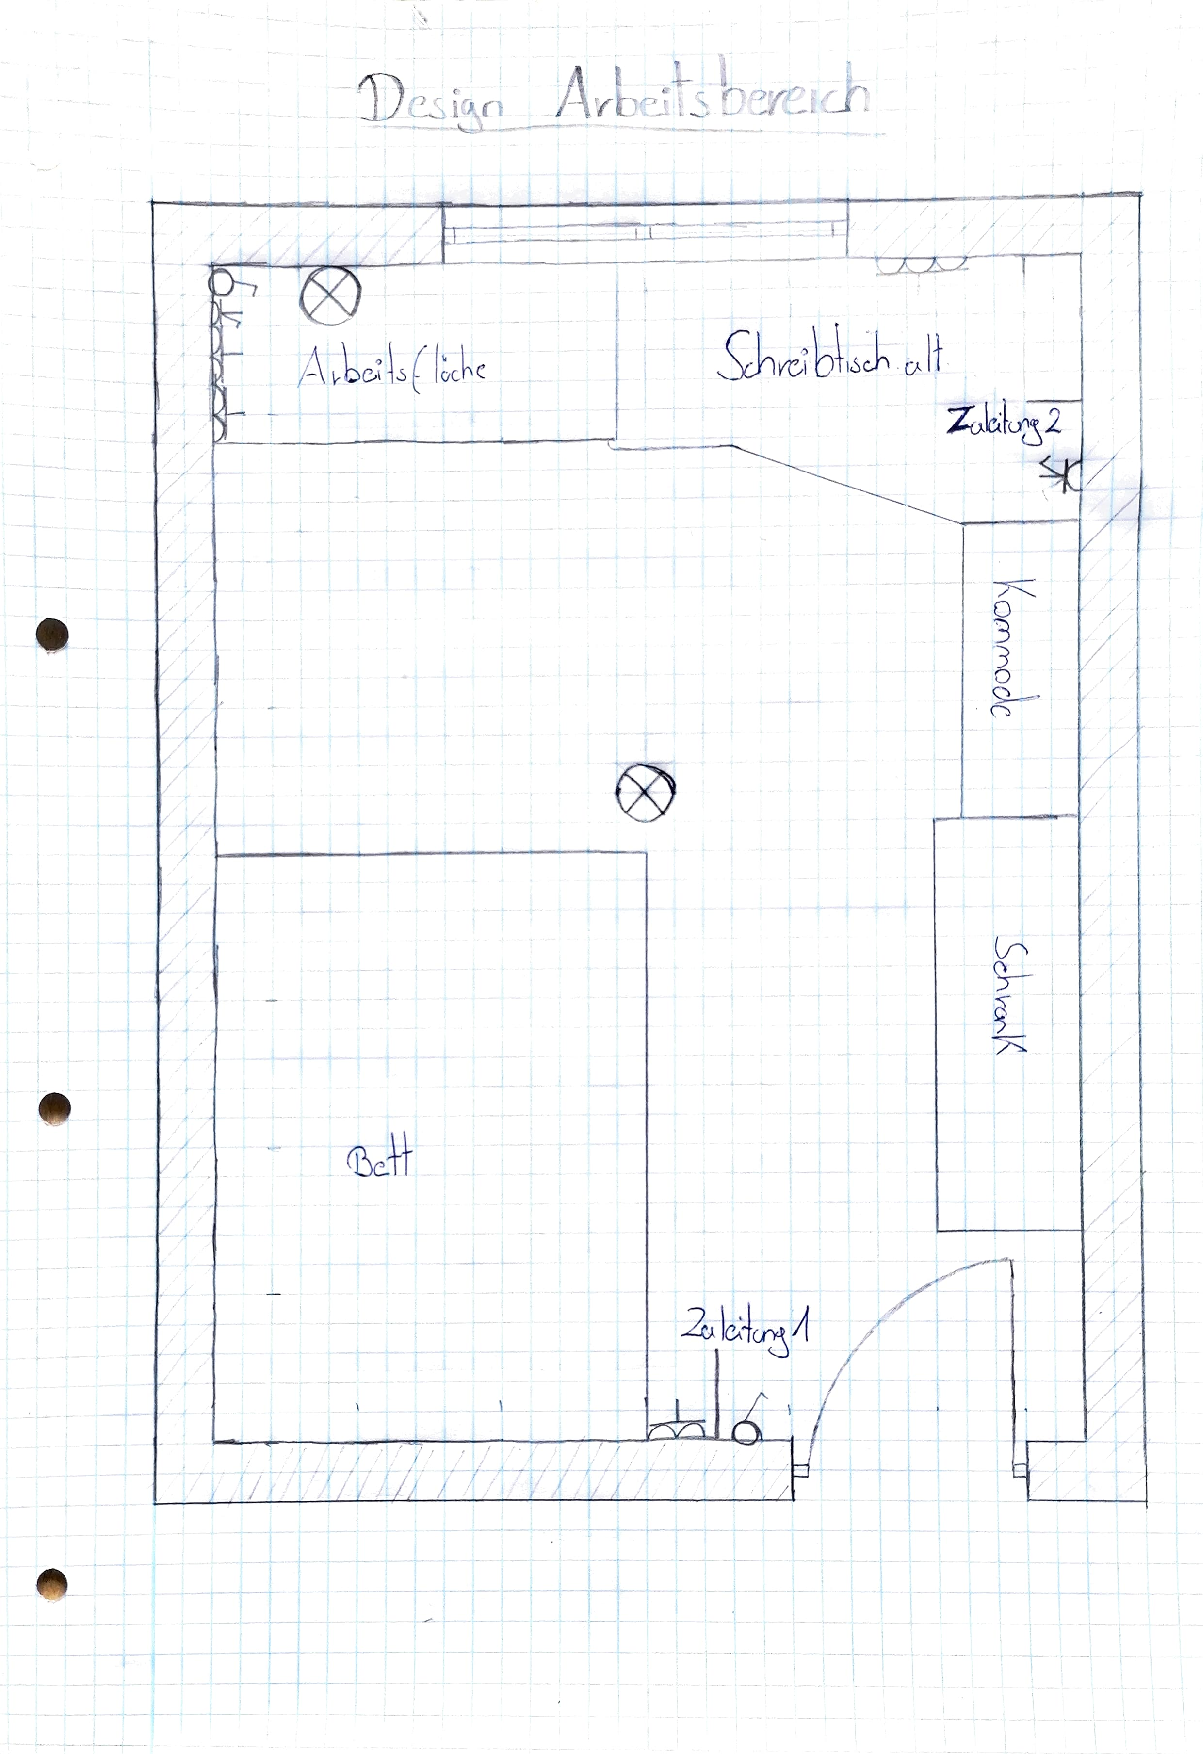
\includepdf[pages=-]{files/layout.pdf}
\section{Design}

Als wichtigste Grundlage für einen funktionellen Arbeitsbereich wurde eine Verbindung zum Stromnetz angesehen.
Hierfür wurde der vorhergehende Installationsplan gezeichnet (siehe vorherige Seite).

Die Einrichtung des Stormnetzes war auch eine der herausfordernsten Aufgaben, 
da ursprünglich nur Zuleitung 1 existierte und aus ästhetischen Grunden von einer Verlegung auf Putz abzusehen war.
Die Lösung hierzu war ein Durchbruch aus dem Nebenzimmer, da in diesem eine Steckdose gegenüberliegend von Zuleitung 2 im Installationsplan vorhanden war.

Die weitere Verlegung erfolgte auf Putz, allerdings unterhalb der beiden Tischplatten.

 Für den Lötkolben wurde eine schaltbare Steckdose installiert, sowie ein Lichtschalter für die Beleuchtung des Arbeitsplatzes, außerdem wurde mehrere Steckdosen zur allgemeinen Nutzung installiert.
